\section{Estudio de Comunidades}

\begin{figure}
    \centering  
    \begin{subfigure}[t]{0.48\textwidth}
      \centering
      \includegraphics[width=\textwidth]{img/resultados/lovaina0.5/communities-size-distribution.png}
      \caption{Coeficiente 0.5.}
    \end{subfigure}
    \vspace{7mm}
    \hfill
    \begin{subfigure}[t]{0.48\textwidth}
      \centering
      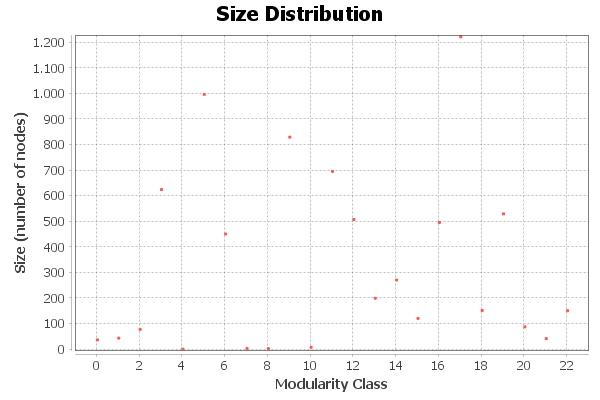
\includegraphics[width=\textwidth]{img/resultados/lovaina1/communities-size-distribution.png}
      \caption{Coeficiente 1.}
    \end{subfigure}
    \hfill
    \begin{subfigure}[t]{0.48\textwidth}
      \centering
      \includegraphics[width=\textwidth]{img/resultados/lovaina2/communities-size-distribution.png}
      \caption{Coeficiente 2.}
    \end{subfigure}
    \hfill
    \begin{subfigure}[t]{0.48\textwidth}
      \centering
      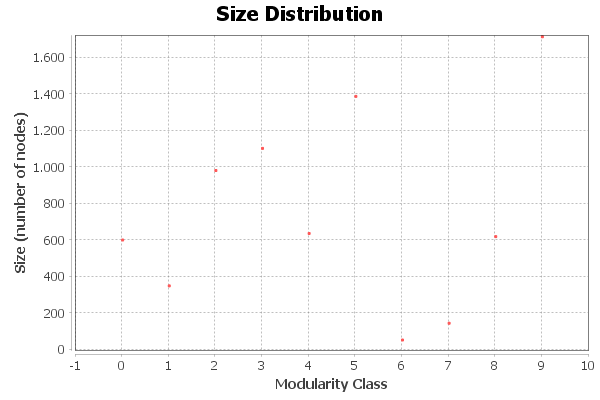
\includegraphics[width=\textwidth]{img/resultados/lovaina3/communities-size-distribution.png}
      \caption{Coeficiente 3.}
    \end{subfigure}
  
    \caption{Gráfico de distribuciones para el algoritmo Lovaina en diferentes coeficientes.}
\end{figure}

\begin{figure}
    \centering  
    \begin{subfigure}[t]{0.48\textwidth}
      \centering
      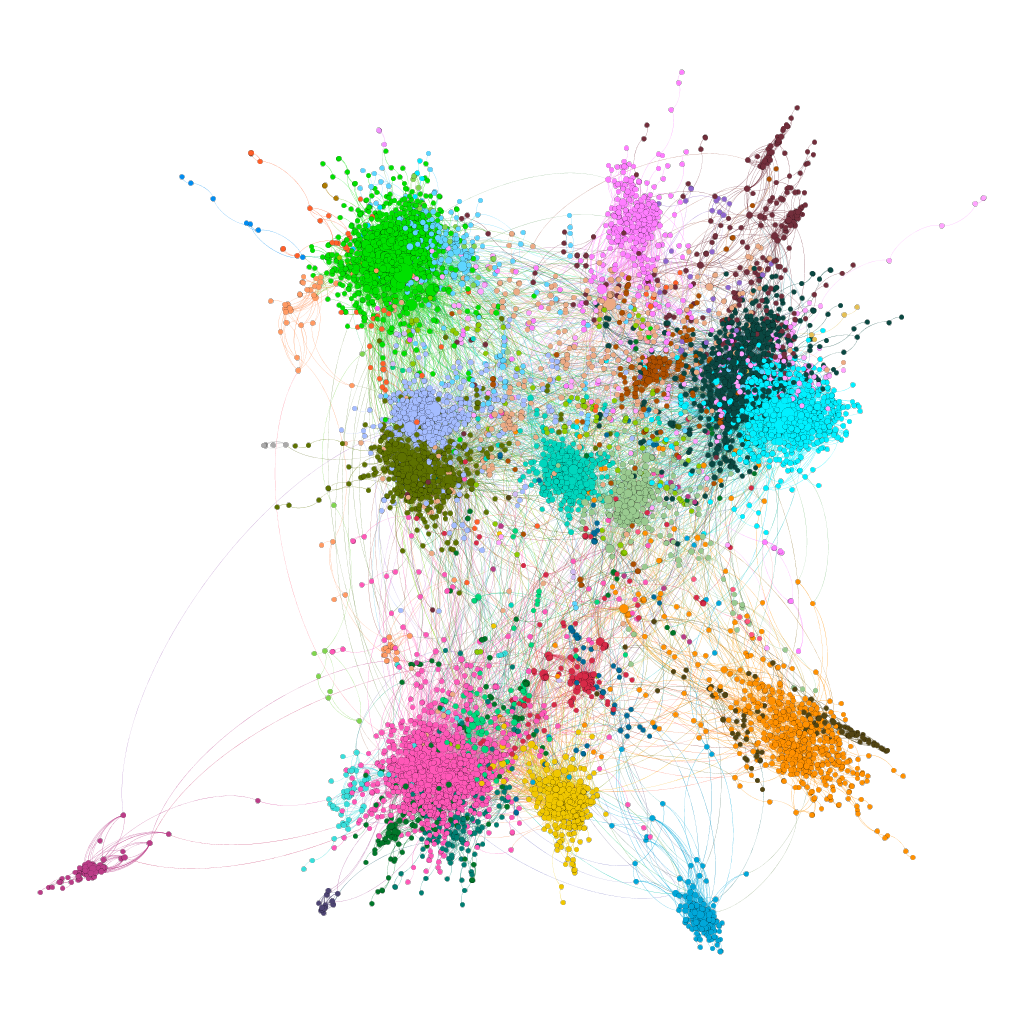
\includegraphics[width=\textwidth]{img/resultados/grado-lovaina0.5.png}
      \caption{Coeficiente 0.5.}
    \end{subfigure}
    \vspace{7mm}
    \hfill
    \begin{subfigure}[t]{0.48\textwidth}
      \centering
      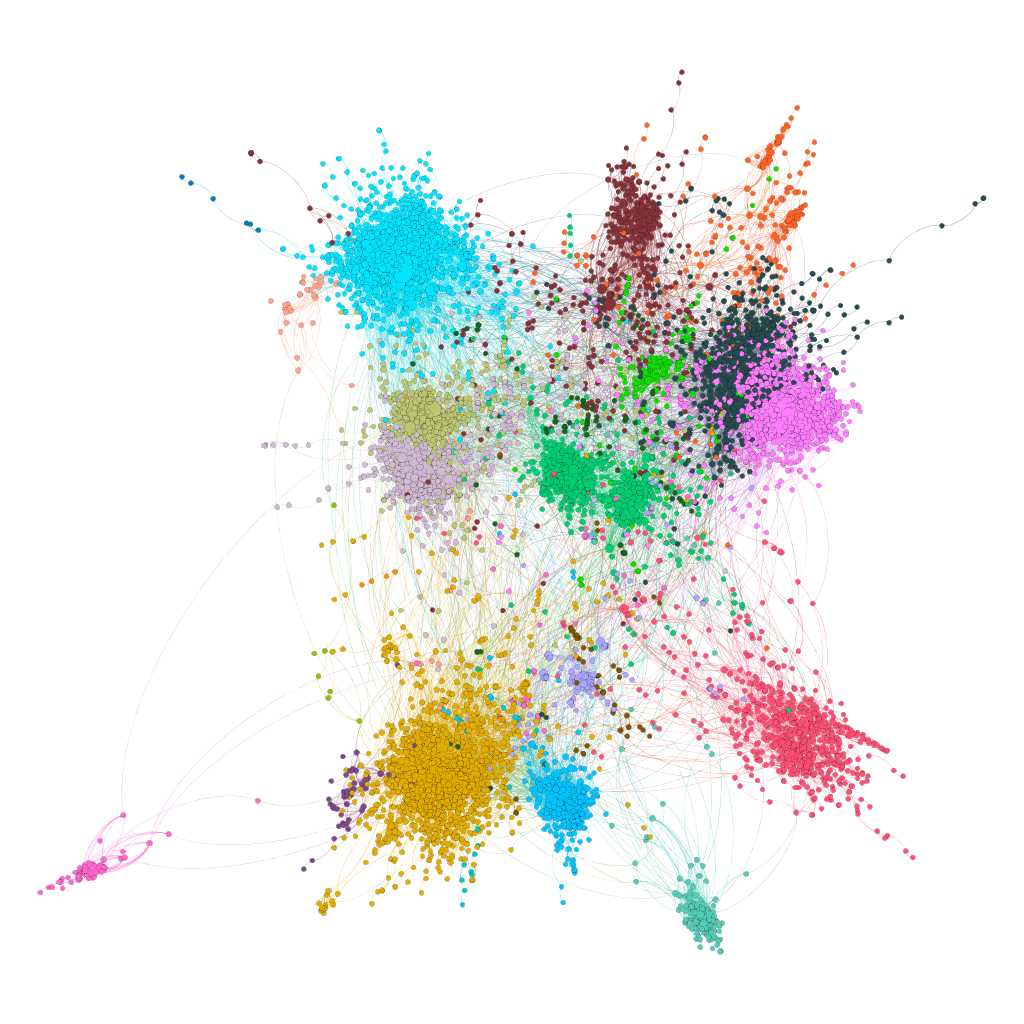
\includegraphics[width=\textwidth]{img/resultados/grado-lovaina1.png}
      \caption{Coeficiente 1.}
    \end{subfigure}
    \hfill
    \begin{subfigure}[t]{0.48\textwidth}
      \centering
      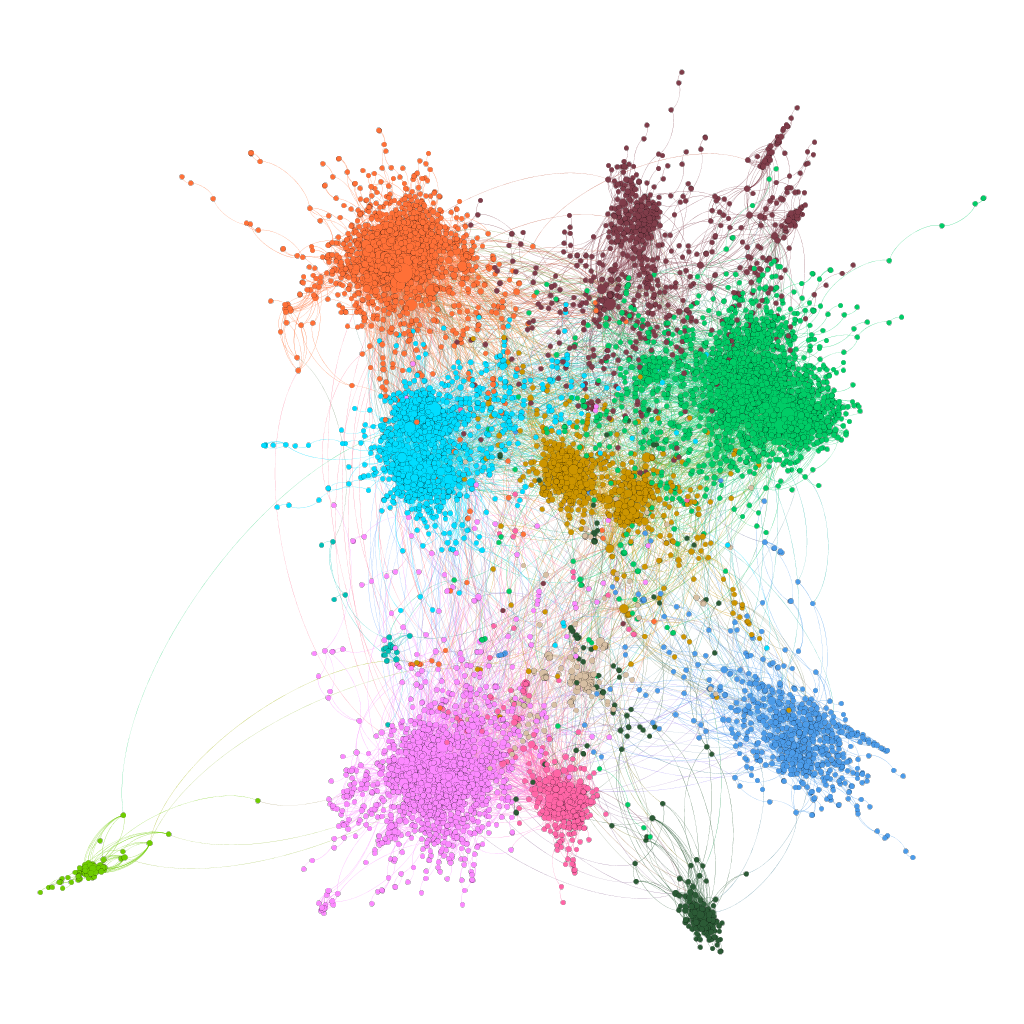
\includegraphics[width=\textwidth]{img/resultados/grado-lovaina2.png}
      \caption{Coeficiente 2.}
    \end{subfigure}
    \hfill
    \begin{subfigure}[t]{0.48\textwidth}
      \centering
      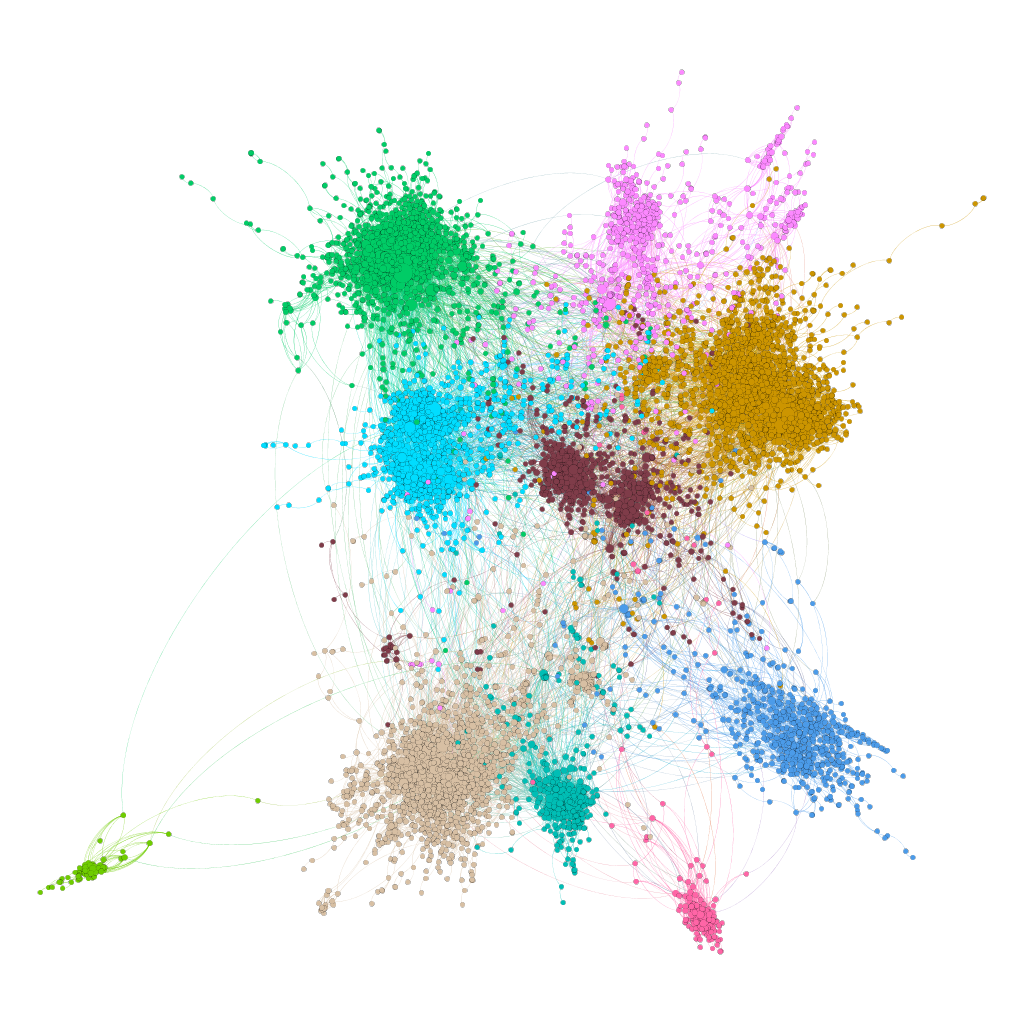
\includegraphics[width=\textwidth]{img/resultados/grado-lovaina3.png}
      \caption{Coeficiente 3.}
    \end{subfigure}
  
    \caption{Comunidades detectadas por el algoritmo Lovaina para diferentes coeficientes.}
\end{figure}

\begin{figure}
    \centering  
    \begin{subfigure}[t]{0.48\textwidth}
      \centering
      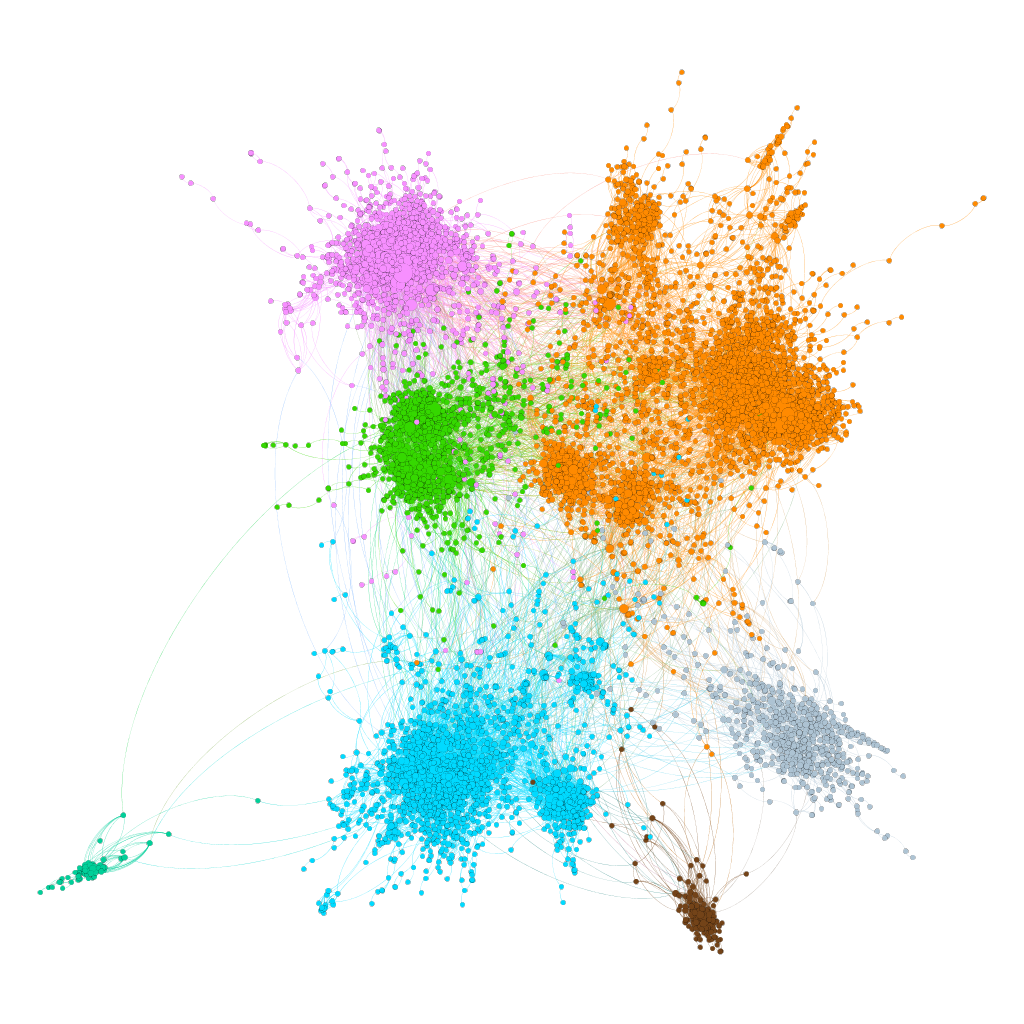
\includegraphics[width=\textwidth]{img/resultados/grado-leinen0.1.png}
      \caption{Coeficiente 0.1.}
    \end{subfigure}
    \vspace{7mm}
    \hfill
    \begin{subfigure}[t]{0.48\textwidth}
      \centering
      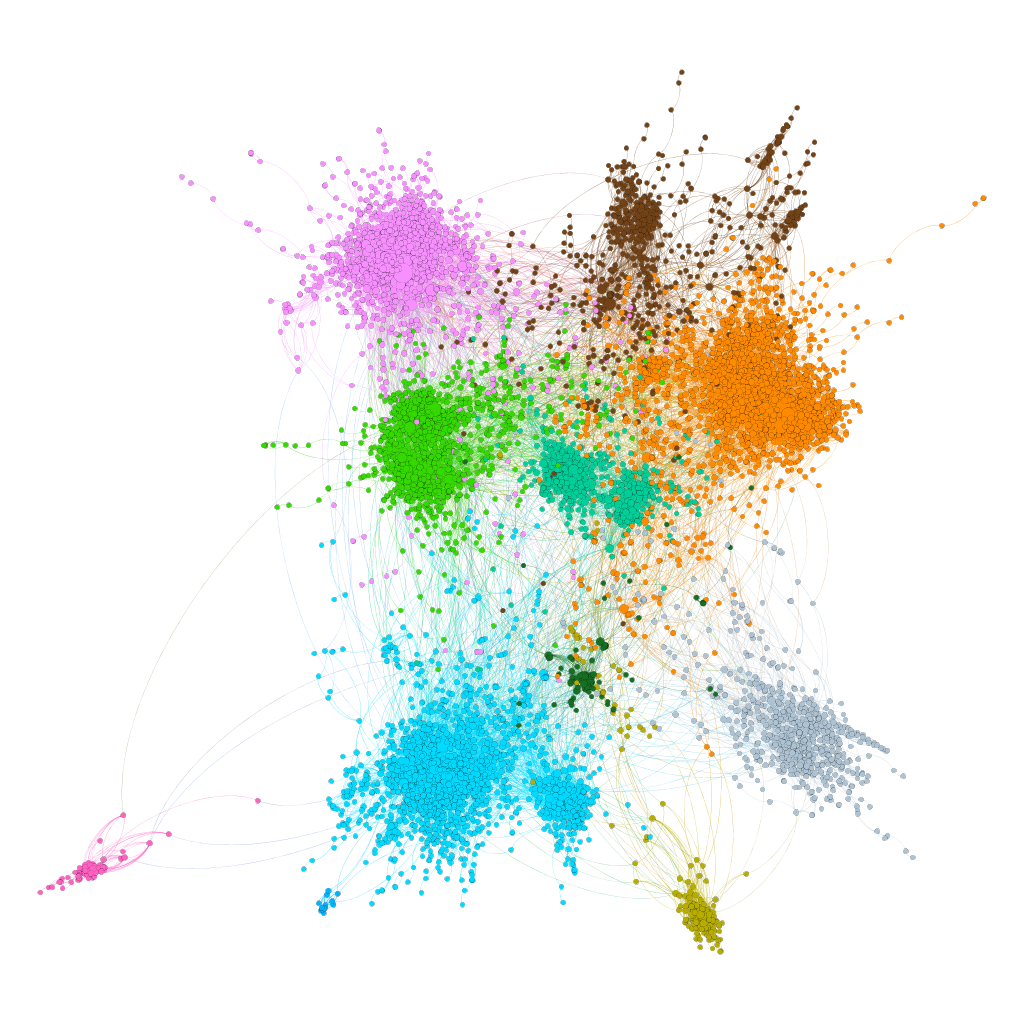
\includegraphics[width=\textwidth]{img/resultados/grado-leinen0.25.png}
      \caption{Coeficiente 0.25.}
    \end{subfigure}
    \hfill
    \begin{subfigure}[t]{0.48\textwidth}
      \centering
      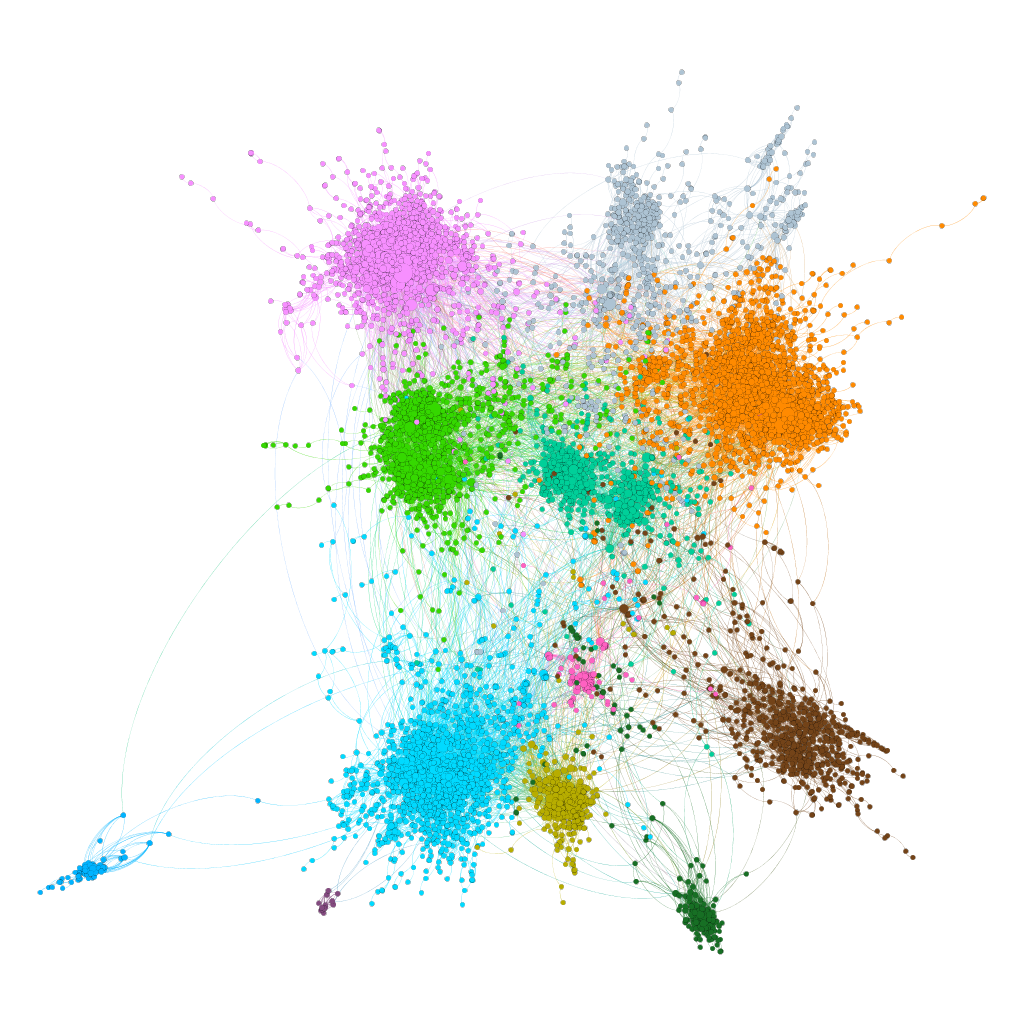
\includegraphics[width=\textwidth]{img/resultados/grado-leinen0.33.png}
      \caption{Coeficiente 0.33.}
    \end{subfigure}
    \hfill
    \begin{subfigure}[t]{0.48\textwidth}
      \centering
      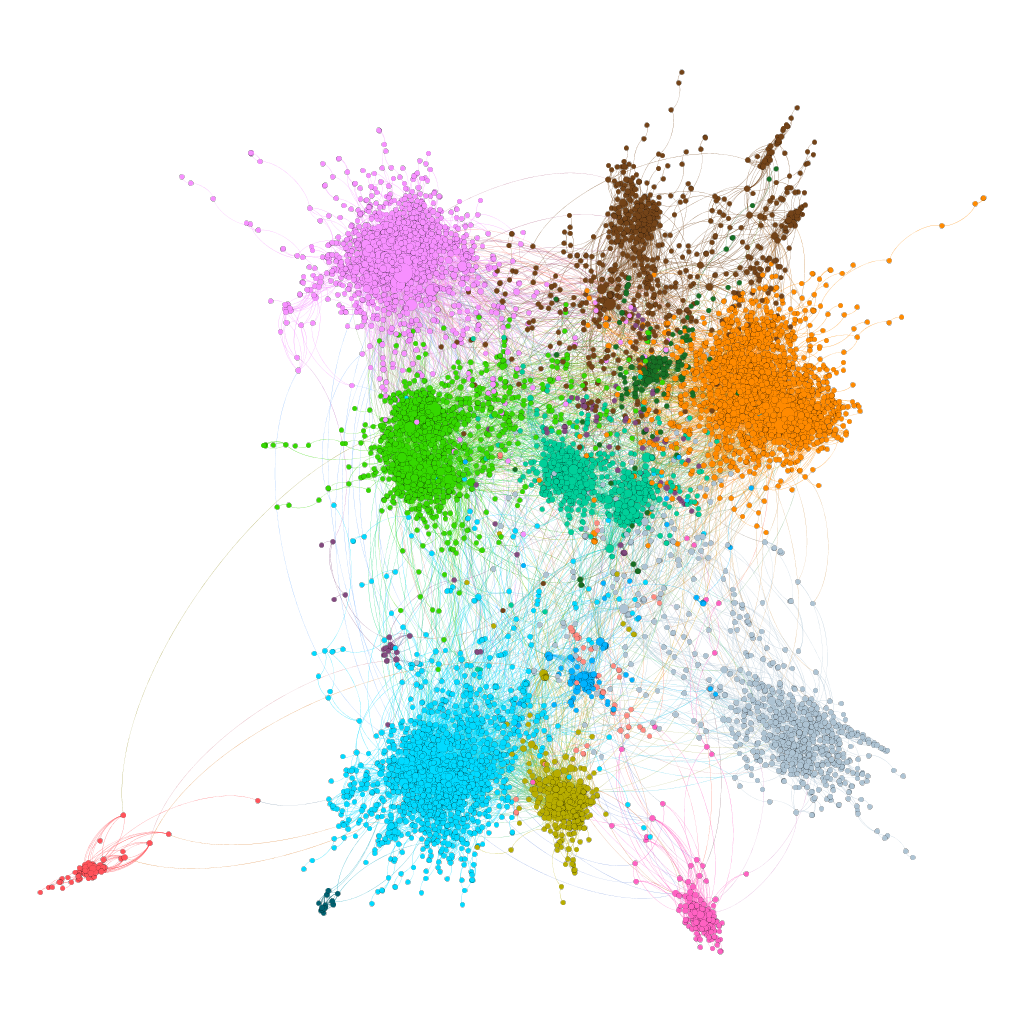
\includegraphics[width=\textwidth]{img/resultados/grado-leinen0.5.png}
      \caption{Coeficiente 0.5.}
    \end{subfigure}
  
    \caption{Comunidades detectadas por el algoritmo Leinen para diferentes coeficientes.}
\end{figure}

La referencia sobre los países puede ser un buen comienzo de partida para la búsqueda de buenas comunidades, pero es importante no dejarse engañar por eso pues por un lado existen hubs de diferentes países altamente conectados entre sí. Además, algunas de las fronteras entre los hubs de los países son difusas y existen zonas de baja conectividad fuertemente intermezcladas.